\chapter{Decision Boundaries}
\label{Chapter4} % Change X to a consecutive number; for referencing this chapter elsewhere, use \ref{Chapter4}

\section{decision boundary definitions} 
%%%%%%%%%%%%%%%%%
\section{The Argmax Function}

A central issue when writing classifiers is mapping from continuous outputs or probabilities to discrete sets of classes. Frequently argmax type functions are used to accomplish this mapping. To discuss decision boundaries, we must precisely define argmax and some of its properties. 

In practice, argmax is not strictly a function, but rather a mapping from the set of outputs or activations from another model into the power set of a discrete set of classes:

\begin{equation}
    \text{argmax} : \R^k \to \mathcal{P}(C)
\end{equation}

Defined this way, we cannot necessarily consider $\argmax$ to be a function in general as the singleton outputs of argmax overlap in an undefined way with other sets from the power set. However, if we restrict our domain carefully, we can identify certain properties. 

Restricting to only the pre-image of the singletons, it should be clear that argmax is continuous. 

Indeed, restricted to the pre-image of any set in the power-set, argmax is continuous. 

Further, we can directly prove that the pre-image of an individual singleton is open. Observe that for any point whose image is a singleton, one element of the domain vector must exceed the others by $\varepsilon > 0$. We shall use the $\ell^1$ metric for distance, and thus if we restrict ourselves to a ball of radius $\varepsilon$, then all elements inside this ball will have that element still larger than the rest and thus map to the same singleton under argmax. Since the union of infinitely many open sets is open in $\R^k$, the union of all singleton pre-images is an open set. Conveniently this also provides proof that the union of all of the non-singleton sets in $\mathcal{P}(C)$ is a closed set. We will call this closed set the argmax Decision Boundary. 

Note : there are ways argmax can be forced to break ties, i.e. by ordering the 

Questions:

Is the decision boundary connected


\section{Defining Decision Boundaries}

\subsection{Complement Definition}

A point $x$ is in the \emph{decision interior} $D_f'$ for a classifier $f: \mathbb{R}^N -> \mathcal{C}$ if there exists $\delta > 0$ such that $\forall \epsilon < \delta$, $|f(B_\epsilon(x))| = 1$. 

The \emph{decision boundary} of a classifier $f$ is the closure of the complement of the decision interior $\overline{\{x : x \notin D_f'\}}$. 

\subsection{Constructive Definition}

A point $x$ is on the \emph{decision boundary} $D$ of a classifier $f$ if $\forall \epsilon > 0$, $|f(B_\epsilon(x))| \geq 2$.\\

A point $x$ is a \emph{binary decision point} if $\exists \delta > 0$ such that $\forall \epsilon > 0$ if $\epsilon < \delta$, then $|f(B_\epsilon(x))| = 2$. 

A point $x$ is on the \emph{$K$-decision boundary} $D^K$ of a classifier $f$ if $\exists \delta > 0$ such that $\forall \epsilon > 0$ if $\epsilon < \delta$, then $|f(B_\epsilon(x))| = K$. 

\subsection{Level Set Definition}

The decision boundary $D$ of a probability valued function $F$ is a union of all level sets $L_{c_1, c_2, a}$ defined by two classes $c_1$ and $c_2$ and a constant $a$ which satisfy two properties: First, given $x \in L_{c_1, c_2, a}$, $F(x)_{c_1} = F(x)_{c_2} = a$ where $a$ is a constant also defining the level set. Second, for all $c \notin \{c_1, c_2\}$, we have $a > F(x)_c$.   

\subsection{Images of Decision Boundaries}

We can consider a classification workflow $f$ from a data space $X$ (e.g. $\mathbb{R}^N$) using a model $F$ mapping the data space $X$ to a probability space $Y$ (e.g. $[0,1]^K$ where $K$ is the number of classes) and using argmax to convert continuous representations in $Y$ to discrete classes in the set of classes $\mathbb{C}$. 

\begin{align}
    X \myrightarrow{F} Y \myrightarrow{\text{argmax}} \mathcal{C}
\end{align}

In this way we define a usual discrete classifier $f = F \circ \text{argmax}$ 

The decision boundary $D$ is defined on $X$, however we may look at the image of the decision boundary under $F$. For example, if there are only two classes, then $Y = [0,1]^2$ and the decision boundary can be nicely visualized by the black line below: 

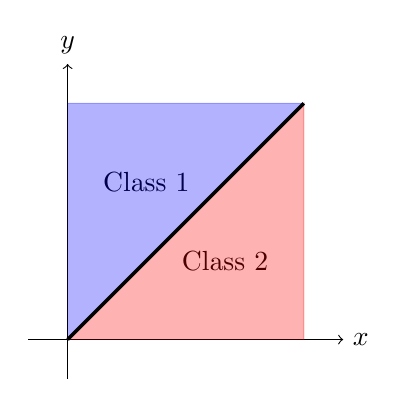
\begin{tikzpicture}
  \draw[->] (-0.5, 0) -- (3.5, 0) node[right] {$x$};
  \draw[->] (0, -0.5) -- (0, 3.5) node[above] {$y$};
  \node at (1, 2) (c1) {Class 1};
  \node at (2, 1) (c2) {Class 2};
  \draw[-, fill, blue, opacity=.3] (0, 3) -- (3, 3) -- (0, 0);
  \draw[-, fill, red, opacity=.3] (3, 0) -- (3, 3) -- (0, 0);
  \draw[scale=1, domain=0:3, smooth, variable=\x, black, line width=0.45mm] plot ({\x}, {\x});
  %\draw[scale=0.5, domain=-3:3, smooth, variable=\y, red]  plot ({\y*\y}, {\y});
\end{tikzpicture}

Furthermore, if the output of $F$ are \emph{probabilities} which add to one, then all points of $x$ will map to the orange line:

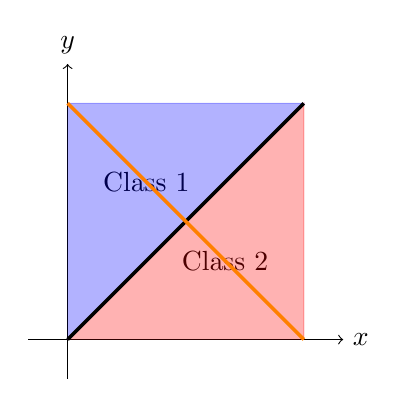
\begin{tikzpicture}
  \draw[->] (-0.5, 0) -- (3.5, 0) node[right] {$x$};
  \draw[->] (0, -0.5) -- (0, 3.5) node[above] {$y$};
  \node at (1, 2) (c1) {Class 1};
  \node at (2, 1) (c2) {Class 2};
  \draw[-, fill, blue, opacity=.3] (0, 3) -- (3, 3) -- (0, 0);
  \draw[-, fill, red, opacity=.3] (3, 0) -- (3, 3) -- (0, 0);
  \draw[scale=1, domain=0:3, smooth, variable=\x, black, line width=0.45mm] plot ({\x}, {\x});
  \draw[-, orange, line width=0.45mm] (0,3) -- (3, 0);
  %\draw[scale=0.5, domain=-3:3, smooth, variable=\y, red]  plot ({\y*\y}, {\y});
\end{tikzpicture}

We note that the point $(0.5, 0.5)$ is therefore the only point on the decision boundary for probability valued $F$. We may generalize to higher dimensions where all probability valued models $F$ will map into the the plane $x + y + z + \cdots = 1$ in $Y$ and the decision boundary will be partitioned into $K-1$ components, where the $K$-decision boundary is the intersection of this plane with the \emph{centroid} line $x = y = z = \cdots$ and the $2$-decision boundaries become planes intersecting at the same line. 

\section{Properties of Decision Boundaries}

In practice, decision boundaries have a variety of properties. The
decision boundary is a pre-image under an onto function that is not
1-1, which allows decision boundaries to vary in upto as many
dimensions as the data space. In practice, this will likely be many
fewer. In particular, decision boundaries should correspond with the
structure of the data. If the data is embedded within a k-manifold
within the input space, the decision boundary can be though of on the
dual space of that manifold.

The dual space of a $k$-manifold embedded in an $n$-dimensional Euclidean space is the space of differential $k$-forms on the manifold. More precisely, for a $k$-manifold $M$ embedded in an $n$-dimensional Euclidean space, the dual space is defined as the space of covariant $k$-tensors on $M$, denoted by $\Lambda^k(M)$, which consists of all linear maps from the tangent space of $M$ at each point to the real numbers.

In particular, when $M$ is a smooth $k$-dimensional manifold, $\Lambda^k(M)$ is the space of smooth $k$-forms on $M$, which can be locally expressed as linear combinations of differential forms of the form $dx_I = dx_{i_1} \wedge dx_{i_2} \wedge \cdots \wedge dx_{i_k}$, where the indices $i_1 < i_2 < \cdots < i_k$ denote the coordinates of a $k$-dimensional chart on $M$ and $dx_i$ denotes the differential of the $i$-th coordinate function.

Intuitively, a $k$-form on $M$ assigns to each $k$-dimensional oriented subspace of the tangent space at a point a signed volume, and the space of all such $k$-forms forms the dual space of $M$. This dual space is important in various areas of mathematics and physics, including differential geometry, topology, and gauge theory.

\subsection{Delaunay Decision Boundaries}

The simplest special case within this dual space is a classifier which
is defined using the Voronoi diagram for the dataset. We can use the
voronoi diagram to define a classifier for an arbitrary query point by
simply assigning it the class of the training point whose voronoi cell
contains it. This has several useful properties, though one in
particular stands out.

Given two points $x$ and $y$ in the training set $X$ which define a delaunay
triangulation and its corresponding voronoi diagram (which is the dual
of the delaunay triangulation) we can see that a line connecting $x$ to
$y$ must orthogonally cross the decision boundary -- which is exactly the voronoi
diagram of this dataset.

Proof:
\begin{proof}
Let $x$ and $y$ be two points in a dataset $X$ that share an edge in the Delaunay triangulation for $X$, and let $e$ be the edge they share in the Delaunay graph. Suppose that $e$ is not orthogonal to the face of the Voronoi diagram that $x$ and $y$ share. Then there exists a point $z$ in the interior of the Voronoi cell for $x$ and $y$ such that the line through $z$ and the midpoint of $e$ intersects the face of the Voronoi diagram at a point $p$.

Since $z$ is in the Voronoi cell for $x$ and $y$, it follows that $d(z, x) < d(z, y)$ (where $d$ is the Euclidean distance). But this contradicts the fact that $x$ and $y$ share an edge in the Delaunay triangulation, which implies that the circumcircle of the triangle formed by $x$, $y$, and $z$ does not contain any other points in $X$. In particular, this means that the circumcenter of this triangle lies on the perpendicular bisector of $e$, which implies that $e$ is orthogonal to the face of the Voronoi diagram that $x$ and $y$ share.

Therefore, we have shown that if $x$ and $y$ share an edge in the Delaunay triangulation for $X$, then the edge they share in the Delaunay graph must be orthogonal to the face of the Voronoi diagram that they share.
\end{proof}
It is immediately clear that for points not in the training set,
the line connecting them with eachother or with a point in the
training set need not cross orthogonal to the voronoi cell
boundaries. In order to talk clearly about such non-orthogonal
crossings, we will define
\begin{definition}
In arbitrary dimensional space, the \emph{angle of incidence} between a line and a plane is defined as the angle between the line and its projection onto the plane, measured in the plane.

More precisely, let $\mathbb{R}^n$ be an $n$-dimensional Euclidean space, let $\ell$ be a line in $\mathbb{R}^n$ with direction vector $\vec{v}$, and let $P$ be a plane in $\mathbb{R}^n$ with normal vector $\vec{n}$. Suppose that $\ell$ intersects $P$ at a point $Q$. Let $H$ be the orthogonal projection of $\ell$ onto $P$, and let $\theta$ be the angle between $\ell$ and $H$.

Then, the angle of incidence between $\ell$ and $P$ is defined as $\alpha = \frac{\pi}{2} - \theta$, where $\pi$ is the constant representing the ratio of the circumference of a circle to its diameter.

Note that when $n=3$, this definition reduces to the familiar definition of the angle of incidence between a line and a plane in three-dimensional space. However, the definition is valid for arbitrary dimensional space.
\end{definition}

and
\begin{definition}
The 
\end{definition}

\subsection{Level Set Definition}
\begin{definition}
The \emph{decision boundary} $D$ of a probability valued function $F$
is a union of all level sets $L_{c_1, c_2, a}$ defined by two classes
$c_1$ and $c_2$ and a constant $a$ which satisfy two properties:
First, given $x \in L_{c_1, c_2, a}$, $F(x)_{c_1} = F(x)_{c_2} = a$
where $a$ is a constant also defining the level set. Second, for all
$c \notin \{c_1, c_2\}$, we have $a > F(x)_c$. This is the
\emph{decision level set} for level $a$. For a given point $x$ on the
decision boundary of a function, the \emph{decision level} is the
value $a$ defining the level set of the decision boundary of which $x$
is a member.

\textbf{Note: } Any point $x$ can be in at most one level set of the
decision boundary. 

\end{definition}

\begin{definition}
  The \emph{dimension} of the decision boundary at a point $x$ is the
  number of dimensions needed to span $\{z : (x + z)$ is in the decision
    level $a$ of the level set containing $x\}$
\end{definition}

A primary property of interest in adversariall attacks is
``sharpness'' i.e. the property that a partition of a set which is
attributed to one class might stab needle-like into a partition of
another set. We will investigate this ``sharpness'' concept by
examining both the incident angle (the acuteness of angles in the
decision boundary) and the dimension of the decision boundary, since
both properties behave like one another. 

There is one conditional bound which is specifically for
voronoi cells which are not exterior to the voronoi diagram. Such
cells are bounded. The line connecting a point within a bounded cell
to the point defining any adjacent voronoi cell.

\subsection{Weighted Delaunay Decision Boundaries}
This simple voronoi classifier has the limitation that it only cares
about which individual training datapoint is closest to the query
point, but is not sensitive to the distribution of this data. If we
suppose that this data is distributed on a manifold with significant
co-dimension with respect to the ambient data space, then it would be
best to use a metric based on this manifold, so that distance among
the data, and hence the delaunay triangulation and the comensurate
voronoi cells would be determined by this metric and thus properly
sensitive to the underlying geometry of this distribution. Alas, this
is akin to having the generating function for nature. It cannot be
computed. So instead, we can take advantage of the Delaunay
triangulation with the usual euclidean metric as an approximation of
the lower dimensional manifold in this case.

This method is limited by the quality of the training dataset as a
sampling of the distribution in question. The Delaunay triangulation
is very sensitive to outliers from a distribution, meaning that our
samples must have relatively little noise in order to be treated as
appropriate samples from the low-dimensional manifold. Second,
Delaunay triangulations are unstable in high-dimensions where very
small triangles are more likely. Both of these problems are lessened
by using data which are sufficiently plentiful relative to the
dimension of the lower dimensional manifold and by requiring that they
do not have more than a small amount of noise to perturb them from the
low dimensional manifold. 

Suppose the lower dimensional manifold $M$ could be defined, and the
training dataset $X$ could be projected onto $M$. The decision
boundary partitioning $M$ would be a set of slices orthogonal to $M$
which would partition any training dataset $X$ into its appropriate
parts. In particular, for a sufficiently dense sampling $x$, we could
define this decision boundary by examining the data points immediately
on either side the decision boundary wherever they meet. We can define
an approximation of the decision boundary as the orthogonal partition
that we expect to be equidistant between adjacent points of different
classes for all samplings of training points. % todo refine this language
In fact, we can define this boundary in the limit using delaunay
triangulation:
\begin{definition}
  Let $M$ be a low dimensional manifold and let $X_{\varepsilon}$ be a
  sampling of points on $M$ for which the maximal edge length along
  its Delaunay triangulation $D_{\varepsilon}$ is
  $\varepsilon$. Given a query point $z$, the $\varepsilon-$Delaunay
  weight for class $i$, $w(z)_i$, is the sum of the barycentric coordinates of $z$
  relative to the vertices with label $i$ of the simplex of $D_{\varepsilon}$ which
  contains $z$. The weight vector $\varepsilon$ boundary level set for
  factor $a$, $B_{\varepsilon,a}$ is the level set $\{z \in M :$ for
  all $i$, we have $w(z)_i \leq a$ and for some $i,j$, $w(z)_i =
  w(z)_j = a\}$. The union of all such level sets over $a$ is the
  \emph{$\varepsilon-$Delaunay-Boundary} $B_{\varepsilon}$. 
  \end{definition}

  Remark, we can extend the decision boundary outside of $M$ by simply
  extending the Delaunay-Boundary using the usual euclidean metric. 

  \begin{theorem}
    Given a low dimensional manifold $M$, 
    \begin{align}
      \lim_{\varepsilon \to 0} B_{\varepsilon}(M) = B(M)
    \end{align}
    $B(M)$ is the decision boundary restricted to $M$. 
  \end{theorem}
  
In this way, a particular training set $X$ defines an approximation of
the general Delaunay Decision Boundary which is well defined outside
of $M$. If the decision boundary is smooth, then for a sufficiently
dense training set $X$ which is sufficiently close to $M$, this
approximation can be bounded by $\varepsilon$ and a lipshitz constant
coming from the mean value theorem on the decision boundary.

It is this approximate form of the decision boundary which we may in
practice evaluate. 

\subsection{Orthant and Wedge}

In order to study decision boundaries, we must talk about properties
related to how decision boundaries interact. We desire a test-object
whose dimensionality and acuteness of angle we can control. To this
end we will use the $k-$dimensional orthant:

\begin{definition}
  Given an integer $k$, the \emph{$k$-orthant} in $n$ dimensions is the set $\{x \in \mathbb{R}^{n}$
  such that for every natural number $i \leq k$, $x_i > 0\}$
  \end{definition}

This concept for an orthant can be extended to be acute in arbitrarily
many angles by tipping toward $x$ to form a wedge.

\begin{definition}
  Given integer $k$ and a set of $k-1$ angles $\Theta$, the \emph{$k-\Theta-$wedge} in $n$ dimensions is the set $\{x \in \mathbb{R}^{n}$
  such that $x_1 > 0$ and for every natural number $1 < i \leq k$,
  $x_i > x_1 \tan(\theta_{i-1})\}$. 
  \end{definition}

These objects allow us to control the dimensionality and acuteness of
a decision boundary to test decision boundary metrics. Another recipe
for analysis is standardizing the paths along which we will cross
decision boundaries. We will use two general paths relative to the
wedge for comparison: centerline and $x-$parallel:

\begin{definition}
  The \emph{centerline} $k-\Theta-$wedge crossing is defined along
  the line $x_1 = t$, for $1 < i \leq k$ $x_i = t
  \tan(\theta_{i-1}/2)$, and for $i > k$ $x_i = 0$.\\

  The \emph{$x-\varepsilon-$parallel} $k-\Theta-$wedge crossing is defined along
  the line $x_1 = t$, for $i > 1$ $x_i = \varepsilon$
\end{definition}

Although we can easily determine whether a point is inside or outside
the wedge simply by checking whether it satisfies the conditions
defining the wedge, we also wish to compute the projection or nearest
point on the wedge for an arbitrary query point. This involves solving
for the closest point to a convex object, which can be accomplished by
projection onto convex sets. 

Computing this projection requires we determine which inequalities
have been violated. Each inequality corresponds with a hyper-plane.
\begin{definition}
  Given a finite set of half-planes $Y_i$ in $\mathbb{R}^n$ and a point $x$,
  let $I$ contain all $i$ such that $x \notin Y_i$. Then since the
  intersection of any number of convex sets is convex, $Y_x = \cap_{i \in
    I} Y_i$ is a convex set. Furthermore, there is exactly one point
  $z$ with $|x - z| \leq |x - y|$ for every $y$ in $Y_x$. This is the
  \emph{projection} of $x$ onto $Y_x$.
\end{definition}

In order to compute this point in practice, we must first determine
all half-planes that do not contain $x$ and then perform orthogonal
projection in sequence along these half-planes using Projection onto
Convex Sets ~/cite{vonneuman-pocs}.

\begin{lemma}
  If all half-planes $Y_i$ with corresponding normal vector $v_i$ have
  boundaries $B(Y_i)$ which are mutually orthogonal, i.e. if $\langle
  v_i, v_j\rangle = 0$ for every combination of $i$ and $j$, then
  the nearest point can be solved by iterative projection 
  \begin{align}
    \vectorproj[v_{i_1}]{(\vectorproj[v_{i_2}]{(\vectorproj[v_{i_3}]{...(x)})})}
  \end{align}
\end{lemma}
(~\cite{vonneuman-pocs})

In the case of the upper wedge, the boundaries are not mutually orthogonal, so
simple orthogonal projection is not sufficient. We must explore this
projection in more detail. Really, what we wish to do is project the
query point $x$ onto the intersection of all of its violated
boundaries. Iteratively, we can orthogonaly project onto the first
hyperplane. We will conduct our projection by subtracting a projection
onto a normal vector for each hyperplane. Given a point $x$, a
hyperplane $p_i$ and its normal vector $v_i$, we define 
\begin{align}
\vectorproj[p_i]{(x)} &= x - x \cdot v_i
\end{align}
The normal vectors for our wedge come in two forms. For the orthant,
all of the normals are of the form $v_i = e_i$. For the angled wedge planes,
they are all of the form $w_i = e_i \cos(\theta_i) - e_1
\sin(\theta_i)$ where $i > 1$. We immediately note that $v_i \cdot v_j
= 0$ for every natural number $i$ and $j$ less than the number of
planes $k$. However,
\begin{align}
  w_i \cdot w_j &= \langle e_i \cos(\theta_i) - e_1 \sin(\theta_i), e_j
                  \cos(\theta_j) - e_1 \sin(\theta_j)\rangle\\
                &= e_ie_j\cos(\theta_i)\cos(\theta_j) -
                  e_1e_j\cos(\theta_j)\sin(\theta_j) - e_1e_i
                  \cos(\theta_i)\sin(\theta_j) +
                  e_1^2\sin(\theta_j)\sin(\theta_i)\\
                &= e_1 \sin(\theta_j)\sin(\theta_i)\\
\end{align}
This means that none of the $w_j$ are orthogonal to each-other and
furthermore 
\begin{align}
  v_1 \cdot w_i &= \langle e_1, -e_1 \sin(\theta_i) + e_i
                  \cos(\theta_i) \rangle \\
                  &= -\sin(\theta_i)
\end{align}
We will leave this latter lack or orthogonality for last, and start by
determining how to sequentially orthogonally project onto the
$w_j$. Critically, we need only project onto the intersection of each
$w_i$ with all previously projected $w_j$. We begin by projecting
from within the plane defined by $w_i$ onto the plane defined by
$w_j$. These vectors are not orthogonal, so we must derive a new
plane and its normal vector $w_{ij}$ which is still orthogonal to $w_i$ but
shares the same intersection with the plane defined by $w_j$ along the
same edge. The conditions that must be satisfied are: 
\begin{align}
  w_{ij} \cdot w_j &= 0 \\
  w_{ij} \perp \cap(w_i, w_j)\\
  w_{ij} \cdot (e_1 + e_i \tan \theta_i + e_j \tan \theta_j) &= 0
\end{align}
This third condition is the requirement that $w_{ij}$ is orthogonal to all
vectors in the intersection of planes $i$ and $j$.

We'll attempt to solve these equations by using a variable $a$ to
account for the discrepency needed to solve these equations. 
\begin{align}
  w_{ij} &= w_j + a = e_j \cos \theta_j - e_1 \sin \theta_j + a\\
  a &= a_1e_1 + a_2e_2 + \cdots a_n e_n \\
  w_{ij} \cdot w_i &= \sin \theta_j\sin\theta_i - a_1 \sin\theta_j +
                     a_i \cos \theta_i = 0\\
  w_{ij} \cdot (e_1 + e_i \tan \theta_i + e_j \tan \theta_j) &= a_1 -
                                                               a_i
                                                               \tan
                                                               \theta_i
                                                               + a_j
                                                               \tan \theta_j
\end{align}
Letting $a_1 \neq 0$ requires that $a = e_1 \sin \theta_j - e_j \cos
\theta_j$ which is a degenerate case, so let $a_1 = 0$. For every
$a_k$ not involved in the intersection of planes, they will have zero
dot product, so we can let them all be 0. Then
\begin{align}
  -a_i \cos \theta_i &= \sin \theta_j \sin \theta_i\\
  a_i &= -\sin \theta_j \tan \theta_i\\
  a_j \tan \theta_j &= \sin \theta_j \tan^2 \theta_i\\
  a_j &= \cos \theta_j \tan^2 \theta_i\\
  w_{ij} &= w_j - e_i \sin \theta_j \tan \theta_i + e_j \cos \theta_j
           \tan^2 \theta_i
\end{align}
Projecting once more onto $w_{k}$ which also shares an intersection
with $w_i$ and $w_j$, we gain one parameter and one degree of
freedom.
\begin{align}
  w_{ijk} &= w_k + a = e_k \cos \theta_k - e_1 \sin \theta_k + a\\
  a &= a_1e_1 + a_2e_2 + \cdots a_n e_n \\
  w_{ijk} \cdot w_i &= \sin \theta_k\sin\theta_i - a_1 \sin\theta_k +
                     a_i \cos \theta_i = 0\\
  w_{ijk} \cdot w_j &= \sin \theta_k\sin\theta_j - a_1 \sin\theta_j +
                     a_j \cos \theta_j = 0\\
  w_{ijk} \cdot (e_1 + e_i \tan \theta_i + e_j \tan \theta_j) &= a_1 +
                                                               a_i
                                                               \tan
                                                               \theta_i
                                                               + a_j
                                                               \tan
                                                                \theta_j
                                                                + a_k
                                                                \tan \theta_k
\end{align}
Now, again letting $a_1 = 0$ to avoid a degenerate case and letting
all other components of $a$ be zero, we have:
\begin{align}
  -a_i \cos \theta_i &= \sin \theta_k \sin \theta_i\\
  a_i &= -\sin \theta_k \tan \theta_i\\
  -a_j \cos \theta_j &= \sin \theta_k \sin \theta_j\\
  a_j &= -\sin \theta_k \tan \theta_j\\
  a_k \tan \theta_k &= \sin \theta_k \tan^2 \theta_i + \sin \theta_k \tan^2 \theta_j\\
  a_k &= \cos \theta_k (\tan^2 \theta_i + \tan^2 \theta_j)\\
  w_{ij} = w_j &- e_i \sin \theta_k \tan \theta_i\\
              &- e_j \sin \theta_k \tan \theta_j\\
              &+ e_k \cos \theta_k (\tan^2 \theta_i + \tan^2 \theta_j)
\end{align}
We see now that we can project an arbitrary sequence of such
intersecting surfaces with each $w_{i...k}$ with $a_i = -\sin \theta_k
\tan \theta_i$ for $i$ less than $k$ and $a_k = \cos \theta_k (\sum_{i
  = 1}^k\tan^2 \theta_i)$. 
Now for our projection algorithm, we first determine if all planes are
satisfied ($x \cdot v_i \geq 0$ and $x \cdot w_i \leq 0$ for every
$i$.) If they are, then we will project onto each plane and pick the
nearest point. If they are not all satisfied, now we'll check each
pair of planes $w_i$ and $v_i$. If both are satisfied, we will skip
them, if both are violated, we will set the coordinate in their native
direction $e_i$ to 0. When only one of the two planes for all compute all planes that are
violated by the position of each query point. For each pair of related
planes $w_i$ and $v_i$, there are three cases. Both satisfied, Both
violated, or either or. In the case that both are violated, i.e. $x
\cdot v_i < 0$, then $x_1 < 0$, which is to say the nearest point
within the wedge in these coordinates will be on the origin. When both
conditions are satisfied, we will ignore this plane except 


%%%%%%%%%%%%%%%%

Now, performing orthogonal projection,
we can orthogonally project in sequence for all half-planes not
containing $x$ except for $v_1$ since $e_1$ is not orthogonal to any
of the wedge planes. Once we have projected onto all other violated
planes, if the projection onto $e_1$ is negative, this will mean that
the nearest point to $x$ is the origin. For $i \neq 1$, all these
projections are of the first form. $x - \sum_{i} x \cdot e_i$. The
first projection of the second form can be done by simple orthogonal
projection, however in order to perform the next projection, we must
project onto the intersection of the two half-planes without leaving
the first plane. We'll need a new plane which is orthogonal to the
first plane, but has the same intersection with the second plane. We
can compute what is missing to make this projection orthogonal. We
have
\begin{align}
  w_i \cdot w_j &= \langle e_i \sin(\theta_i) - e_1 \cos(\theta_i), e_j
                  \sin(\theta_j) - e_1 \cos(\theta_j)\rangle\\
                &= e_ie_j\sin(\theta_i)\sin(\theta_j) -
                  e_1e_j\sin(\theta_j)\cos(\theta_j) - e_1e_i
                  \sin(\theta_i)\cos(\theta_j) +
                  e_1^2\cos(\theta_j)\cos(\theta_i)\\
                &= e_1 \cos(\theta_j)\cos(\theta_i)\\
\end{align}

We can solve for a perturbation in the $e_1$ direction which will make
these two normal vectors orthogonal but due to preserving 




\section{exploring boundary curvature with Random Walks}

To analyze decision boundary curvature, we will project samples of points onto the decision boundary and then use Singular Value Decomposition to analyze the \emph{projected points}. In general, this process will involve first selecting two images $x_1$ and $x_2$ for which $C(x_1) \neq C(x_2)$. A point $x_b$ for which $C(x_b)$ is ambiguous between $C(x_1)$ and $C(x_2)$. The resulting sample $X$ will be projected to the decision boundary by either computing a loss function that is minimized when each of the classes $C(X)$ flip from $C(x_1)$ to $C(x_2)$ or vice versa respectively and performing gradient descent, or by interpolating to the parent point of opposite class (so for $x \in X$, if $C(x) = C(x_1)$, we will interpolate from $x$ to $x_2$). 

Once a projection has been found, we will take the singular value decomposition (SVD) of this sample and examine it for degeneracy. 


Initial comparison of SVDs of decision boundary points yields a single dominant singular value which corresponds with the content of the original image on the boundary. All random noise appears to be mostly orthogonal to this. 

Once this vector is removed, the remaining signal is simply the adversarial attack information. 

To get a set of singular vectors which to not emphasize the image content, we take random differences among the sampled images and take the SVD of those random differences. 

In these first 10 images, this procedure is carried out on the orthant, where samples are generated with mean 0 and are projected onto orthants with increasing numbers of dimensions. We can see a very clear dropped set of singular values smaller than the rest, which indicate the number of degenerate dimensions. In each of these cases, the dropped singular values match the dimension of the orthant. 

Experiment : A valid experiment here is to measure the difference between the images and the projection to get -- in this case -- normal vectors to the orthant for each image sampled. The SVD of these normals can be computed to determine the number of dimensions in the projecetion operation. This same procedure can be caried out later in the real practical image projections, although in that case orthogonality is not guaranteed. 

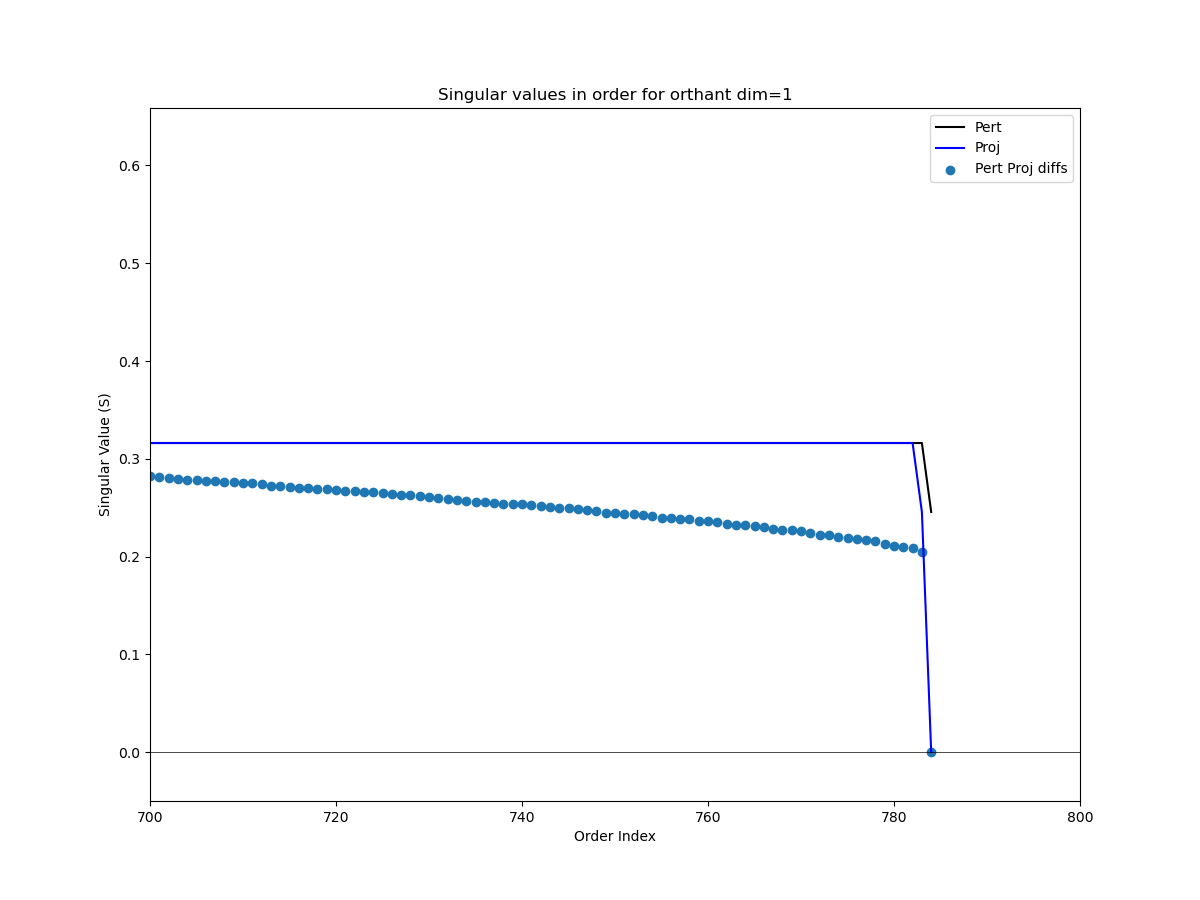
\includegraphics[width=8cm]{c4_figures/e03-SVD-Orthant_origin-dim-cropped1.png}
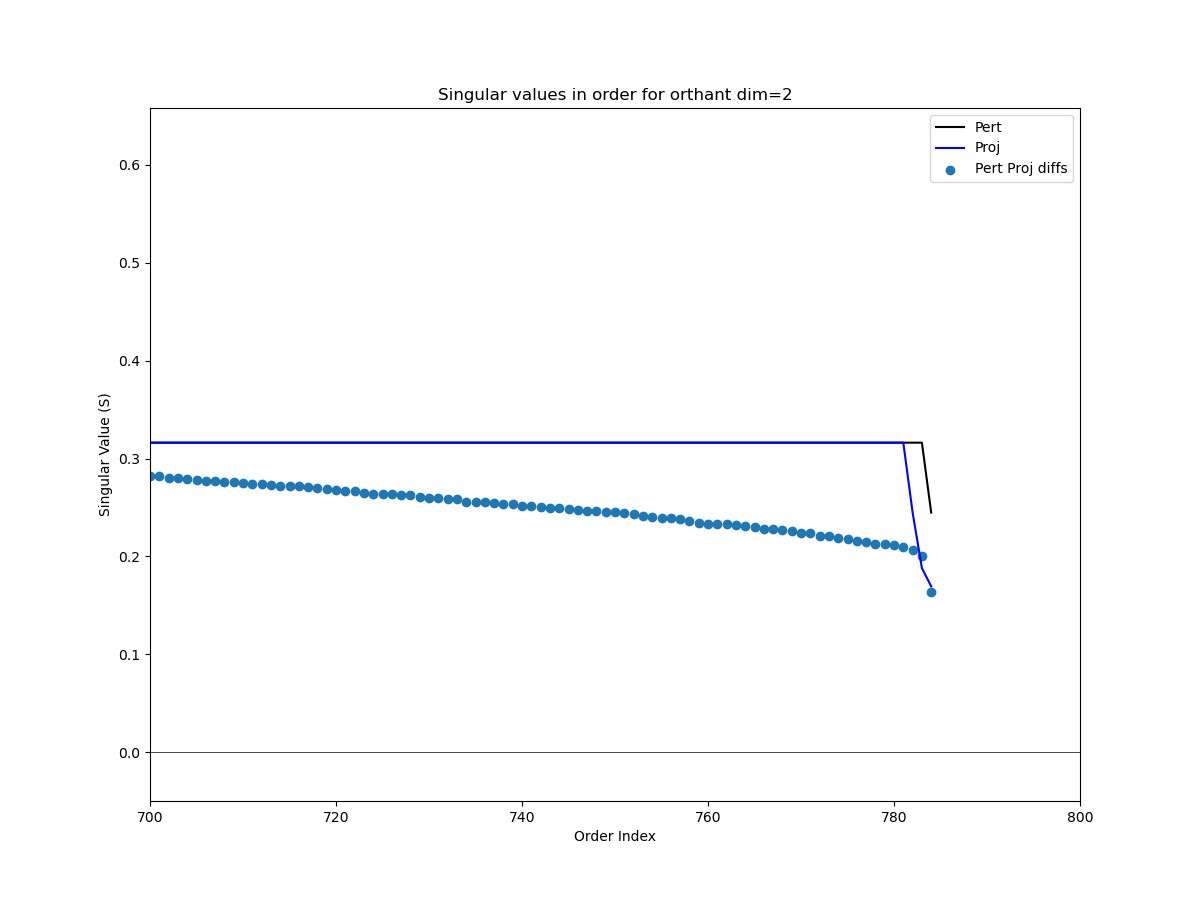
\includegraphics[width=9cm]{c4_figures/e03-SVD-Orthant_origin-dim-cropped2.png}
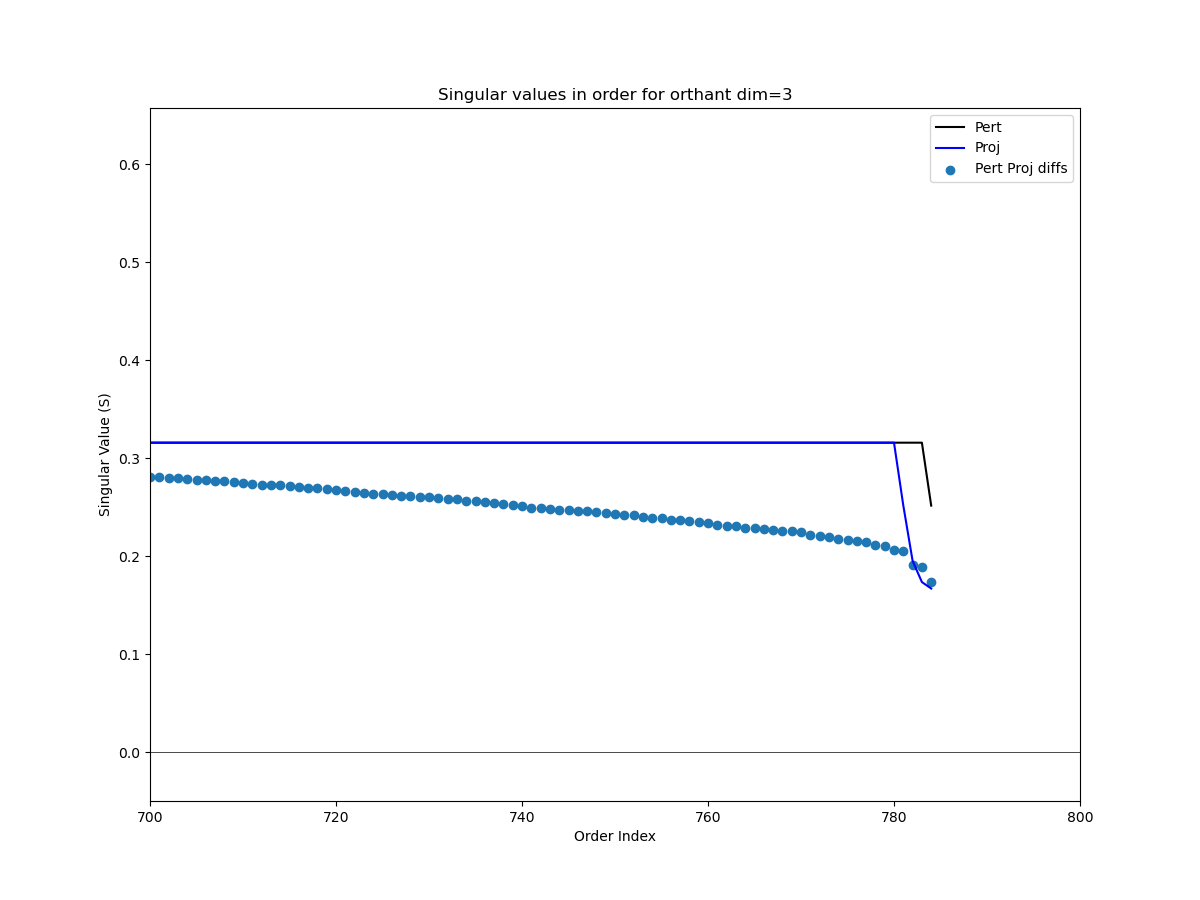
\includegraphics[width=9cm]{c4_figures/e03-SVD-Orthant_origin-dim-cropped3.png}
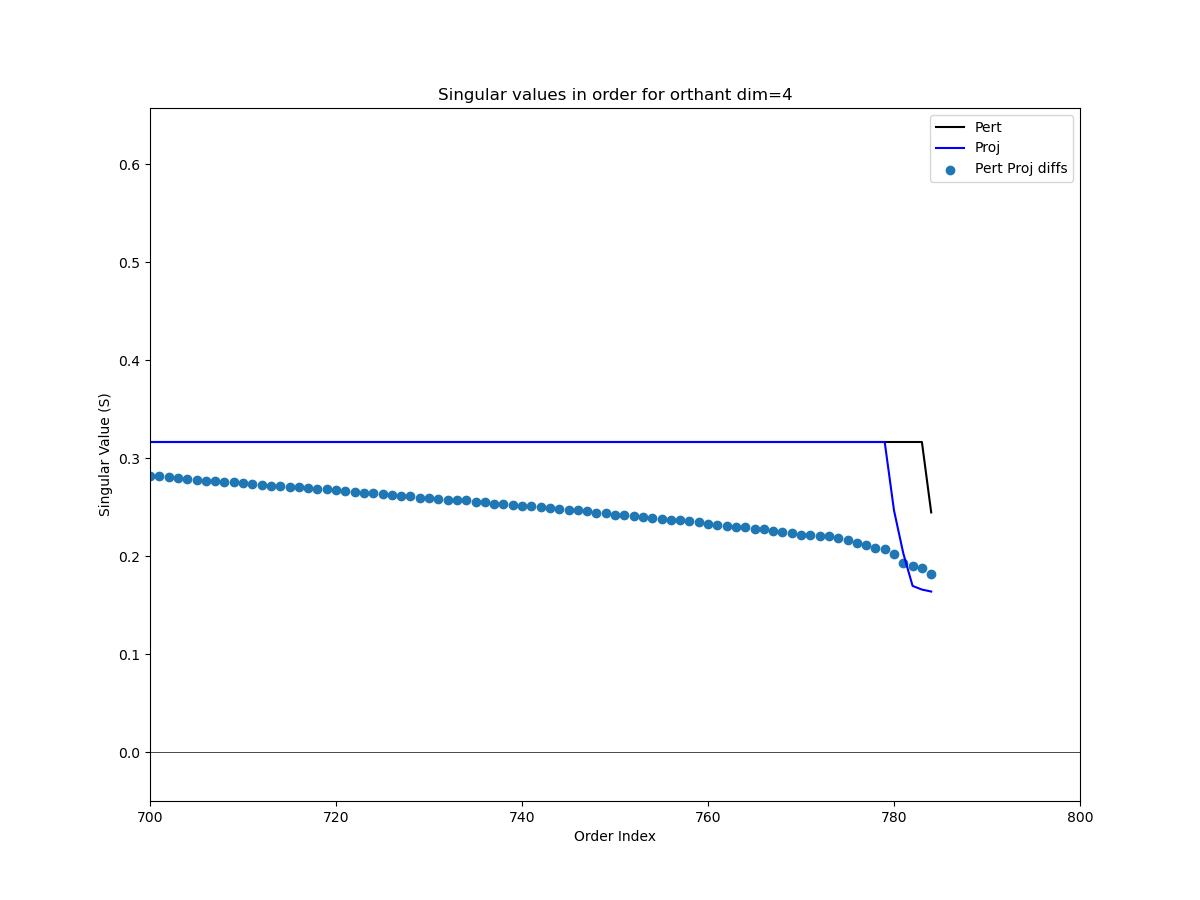
\includegraphics[width=9cm]{c4_figures/e03-SVD-Orthant_origin-dim-cropped4.png}
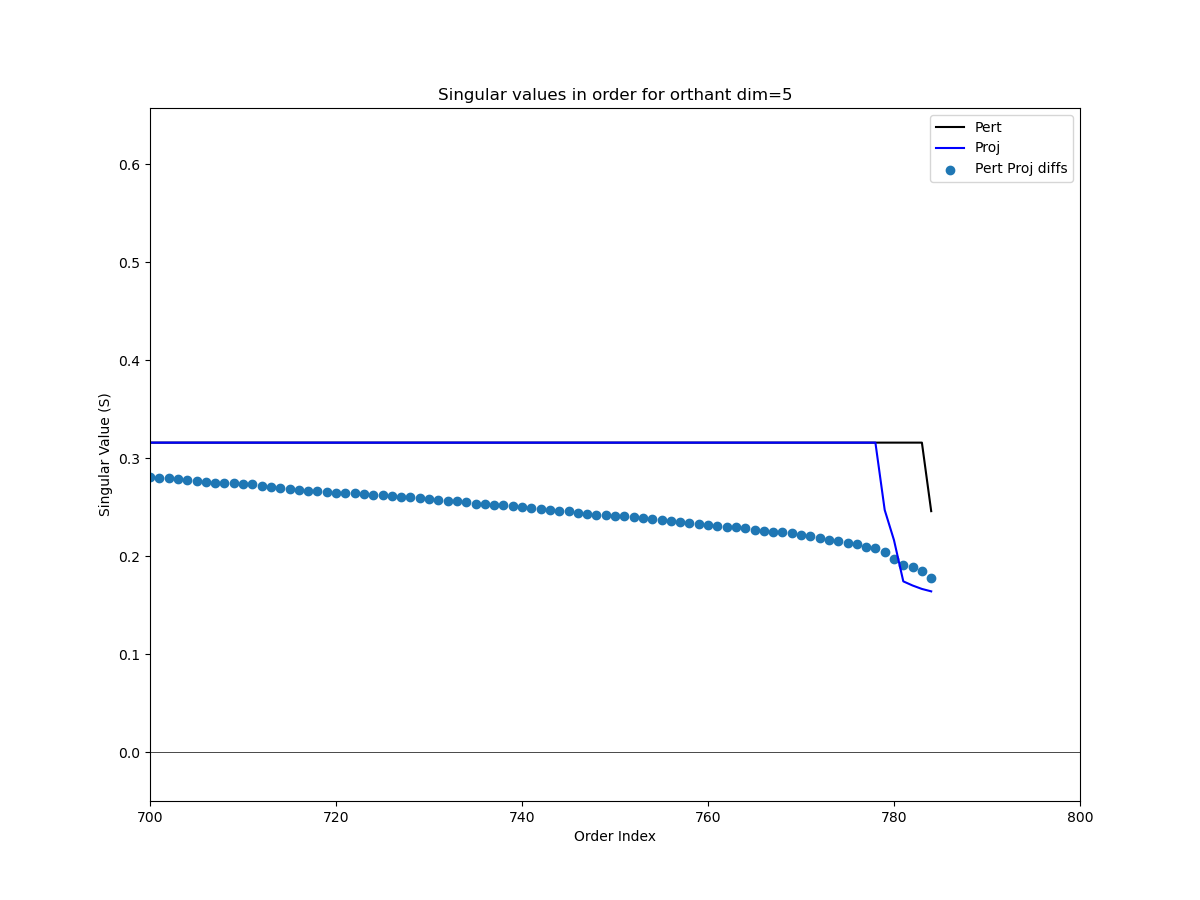
\includegraphics[width=9cm]{c4_figures/e03-SVD-Orthant_origin-dim-cropped5.png}
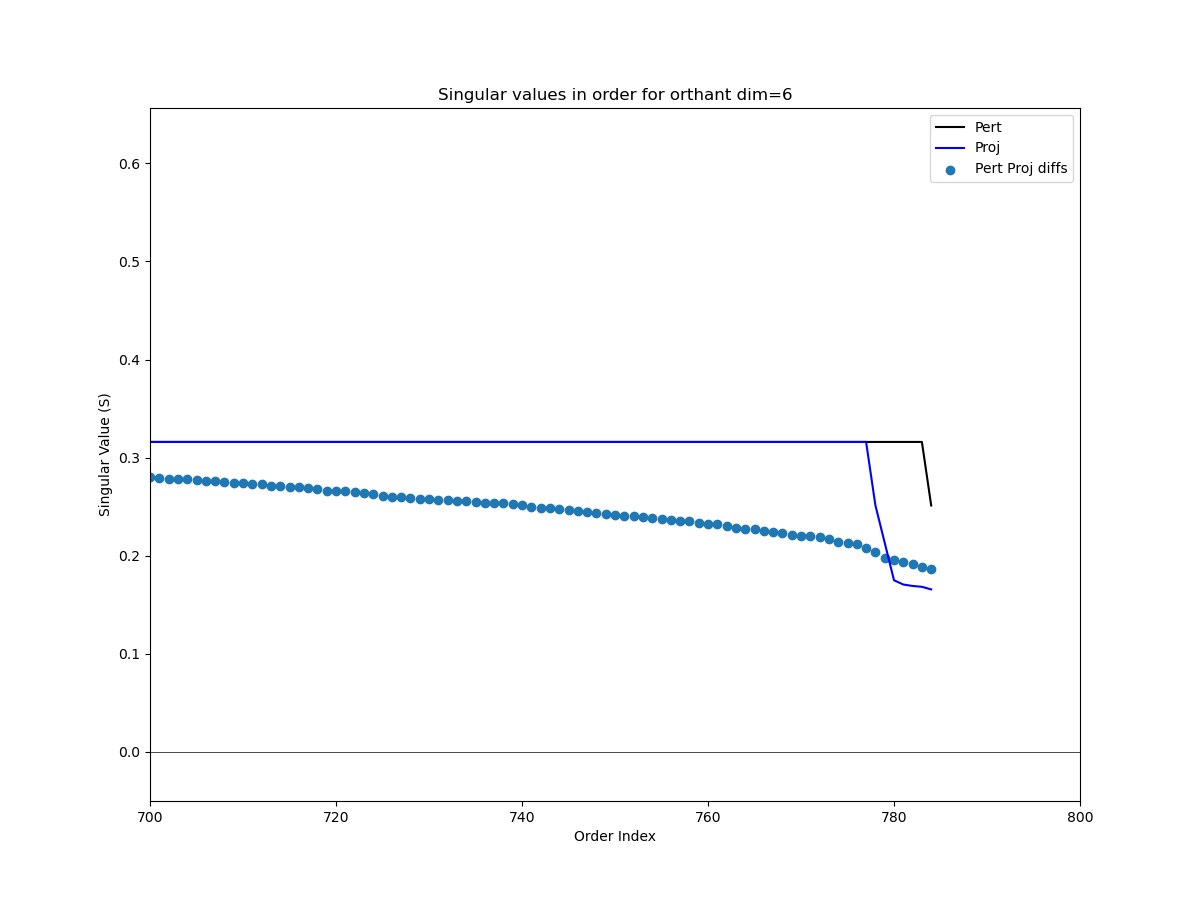
\includegraphics[width=9cm]{c4_figures/e03-SVD-Orthant_origin-dim-cropped6.png}
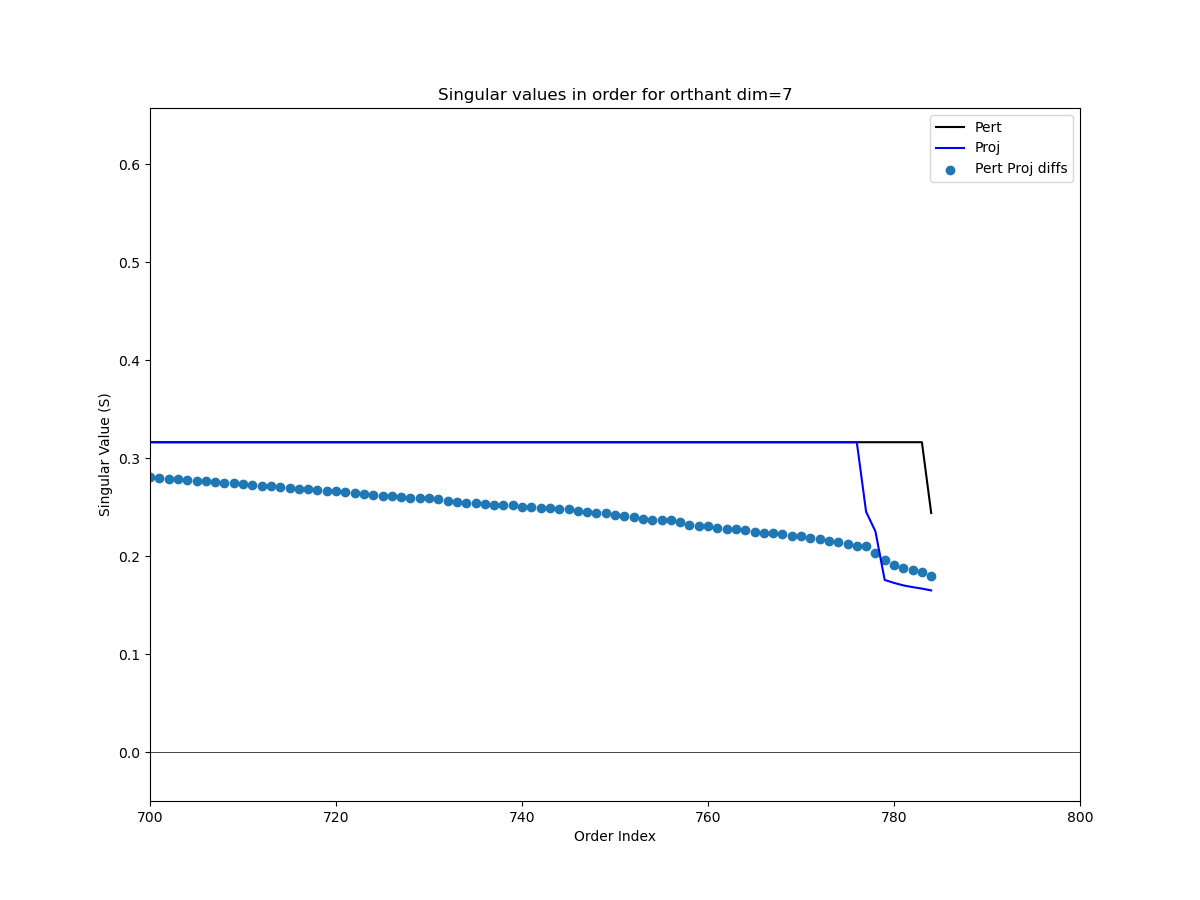
\includegraphics[width=9cm]{c4_figures/e03-SVD-Orthant_origin-dim-cropped7.png}
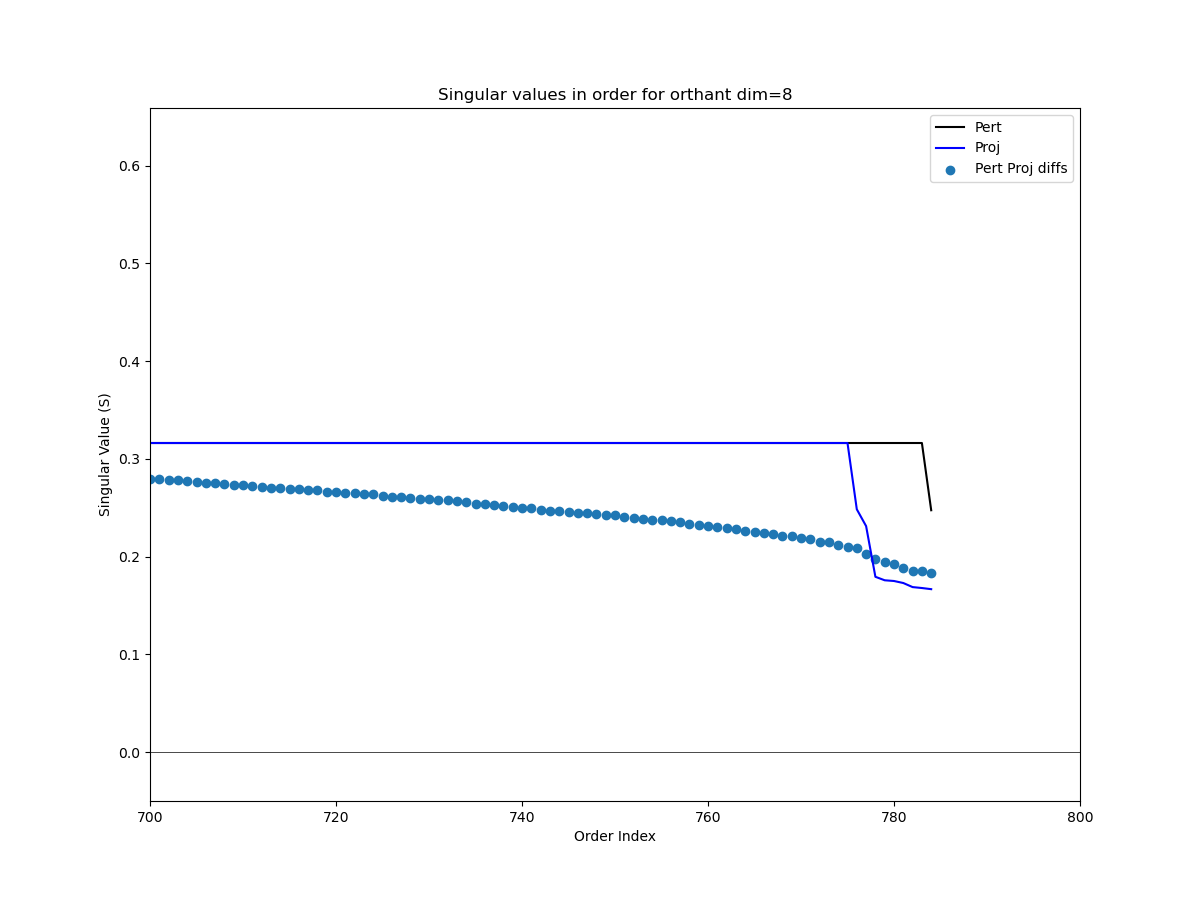
\includegraphics[width=9cm]{c4_figures/e03-SVD-Orthant_origin-dim-cropped8.png}
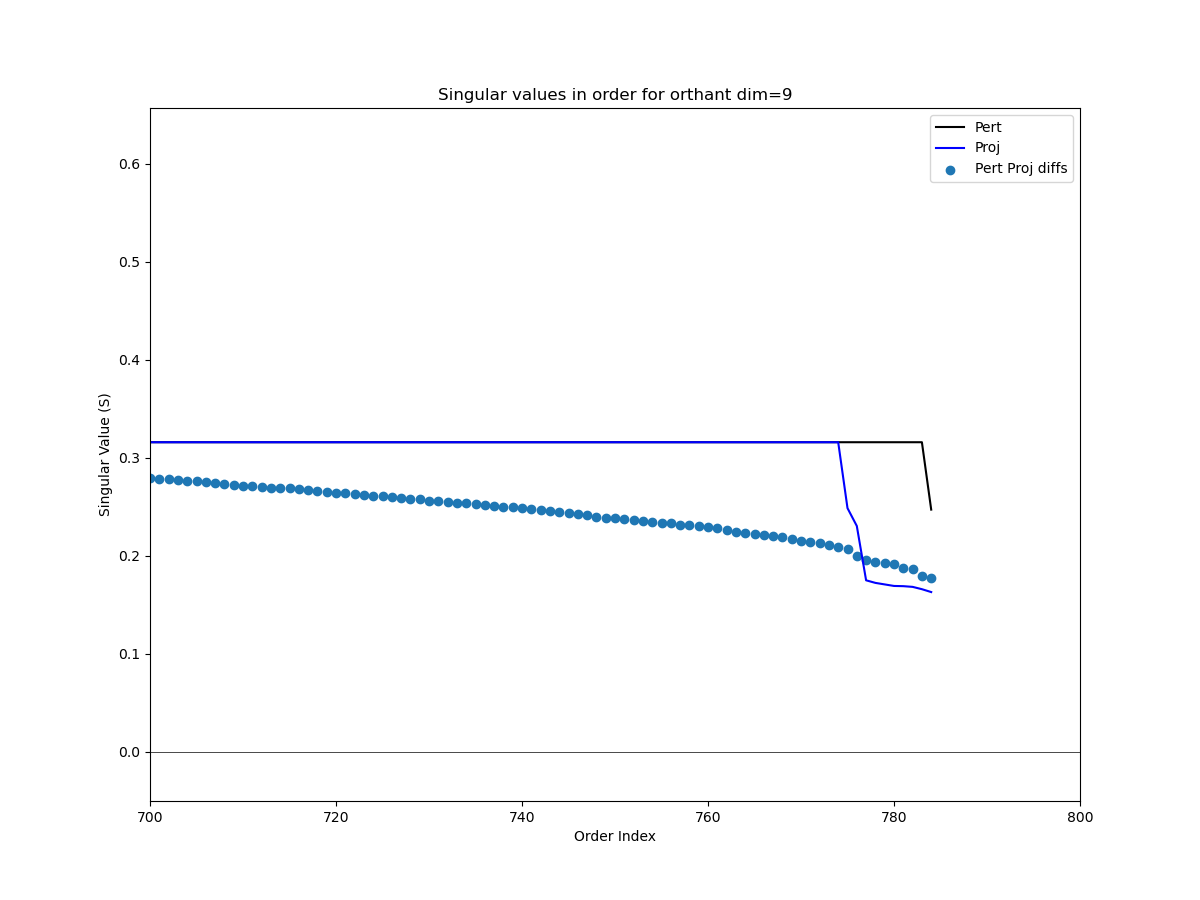
\includegraphics[width=9cm]{c4_figures/e03-SVD-Orthant_origin-dim-cropped9.png}
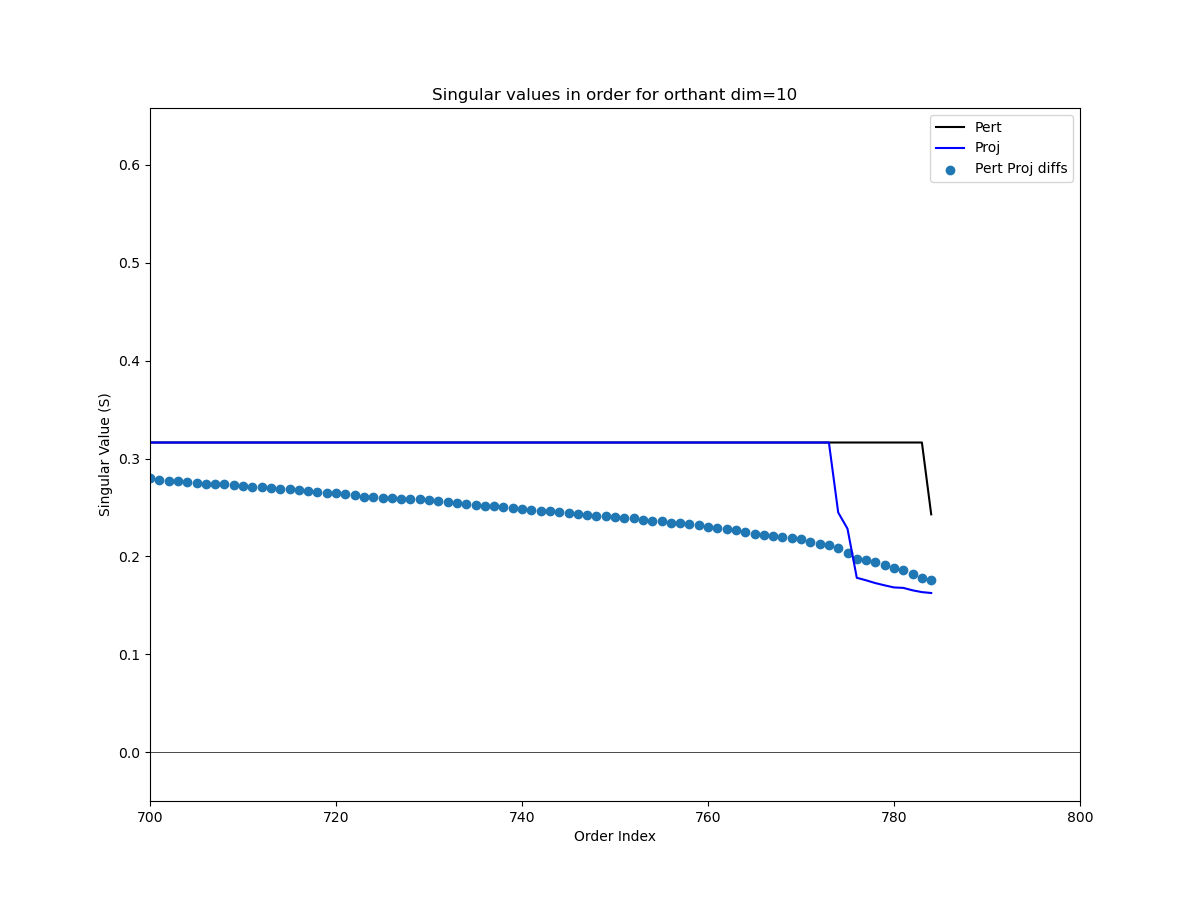
\includegraphics[width=9cm]{c4_figures/e03-SVD-Orthant_origin-dim-cropped10.png}

There is a question of how best to measure "normal" vectors for each projection. The most direct computation is to take a sample with small variance around each point on the decision boundary and solve least squares of each of these samples. We have previously observed that \emph{most} of the decision boundary is locally planar. 

It remains to compare these computed normals with other known quantities, e.g. the gradient computed with respect to adversarial loss functions and the difference between each sampled image and its resultant projection. In addition, it remains to compare the normals of multiple nearby images to determine at what radius of sample the decision boundary begins to show curvature.\\

The following image shows singular values in order for a sample around a decision boundary image in MNIST generated by interpolating from a test image to an adversarial image generated from it. This plot is dominated by the natural distribution of singular values for a gaussian and also by the original image information which can be seen as a huge singular value on the far left. We will address both of these factors in following plots. \\

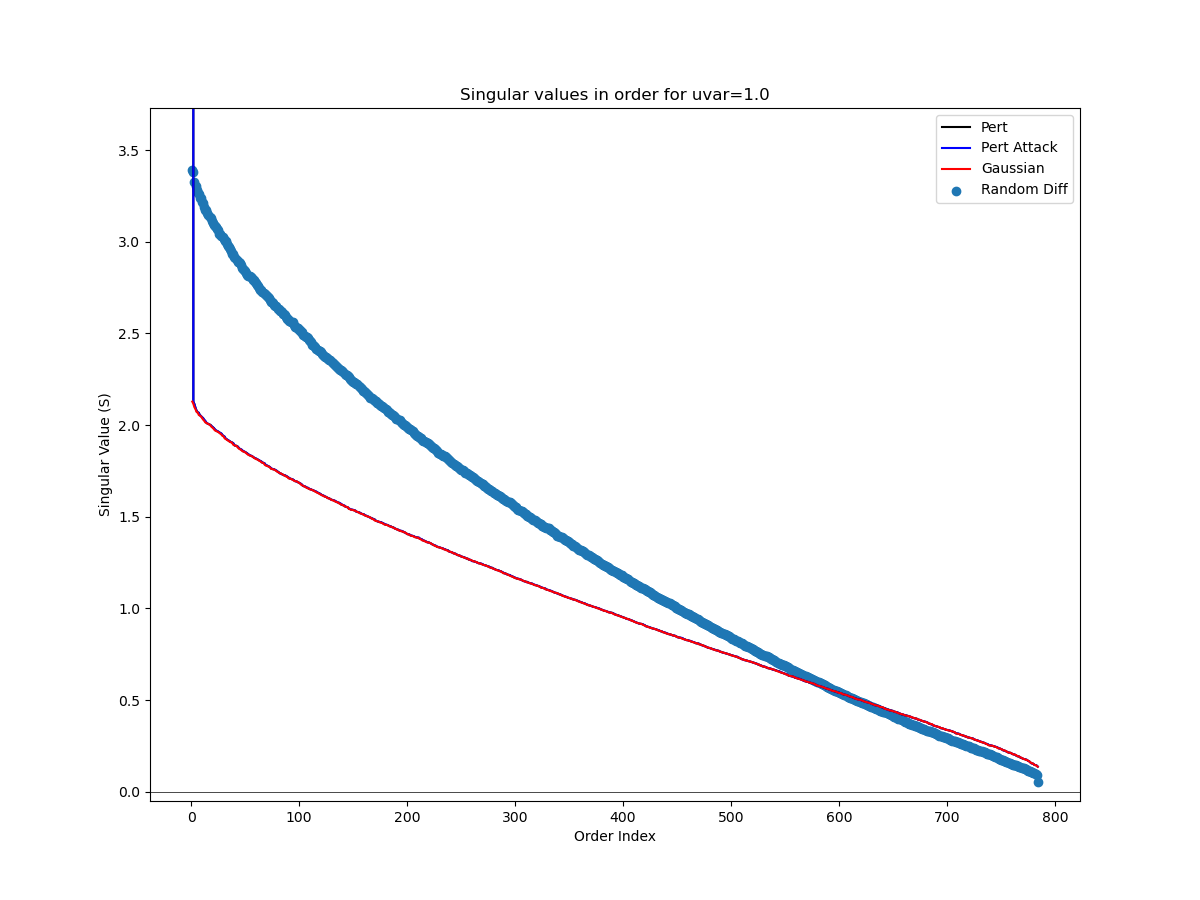
\includegraphics[width=14cm]{c4_figures/SVD-rand_diff-decision_boundary_uvar-1.0-index-0-image-999.png}

The following plots are generated with a new distribution to replace the gaussian. This "Flat SVD" distribution is generated by first taking a gaussian sample representable by a matrix $X$, then taking the SVD of this gaussian sample $U \Sigma V = X$, replacing $\Sigma$ by $|\Sigma|_2 I$. This distribution has the property that its SVD is flat, while maintaining the Frobenius norm of $X$. This helps to highlight degeneracy in singular values. \\

These first two plots are generated by sampling around a decision boundary image found by interpolating between two test images (rather than a test image and an adversarial example generated from it). We note that the SVD contains two degernate values. These seem to correpond with the two original images of the interpolation. 

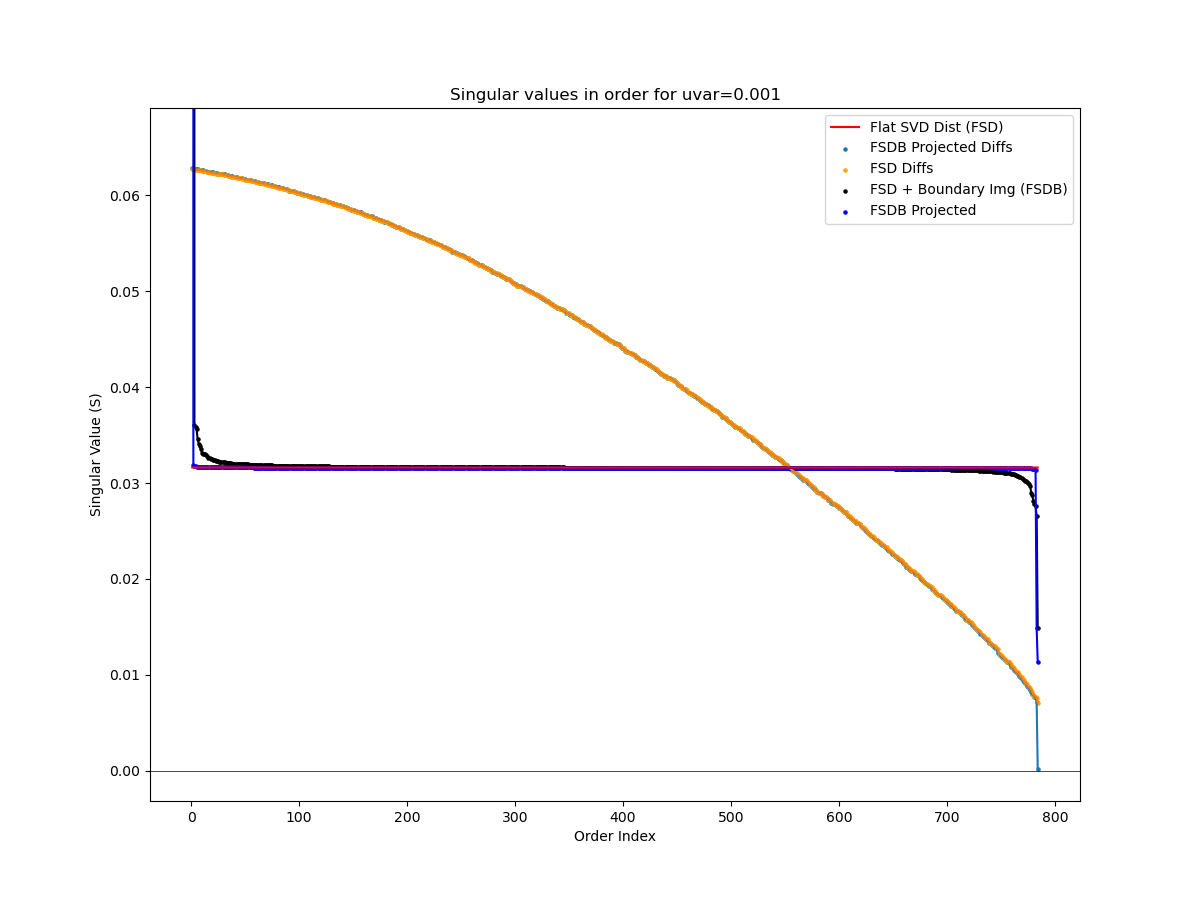
\includegraphics[width=14cm]{c4_figures/e05-SVD-uniform-rand_diff-decision_boundary_uvar-0.001-index-0-image-999.png}

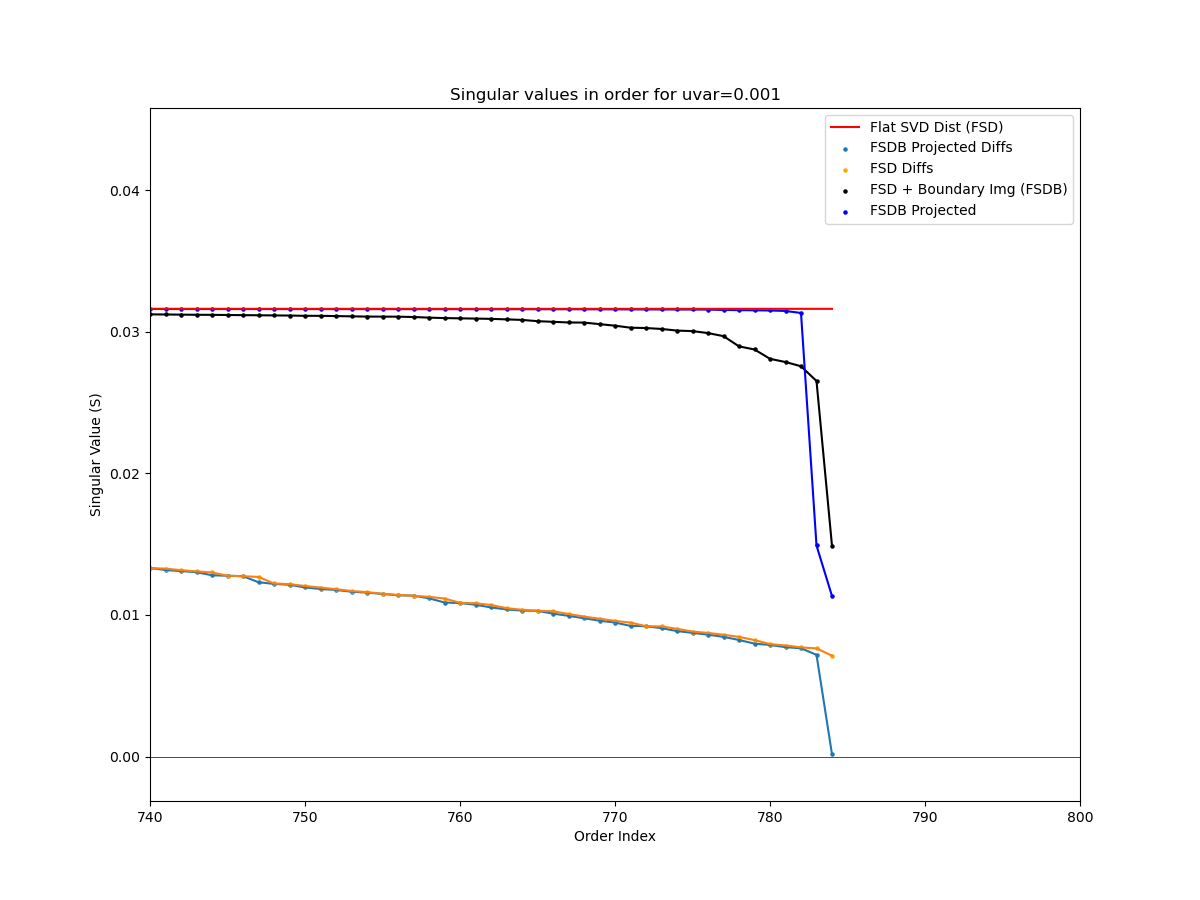
\includegraphics[width=14cm]{c4_figures/e05-SVD-uniform-rand_diff-decision_boundary_uvar-0.001-index-0-image-999-cropped.png}


These last two images are generated with the flattened distribution 

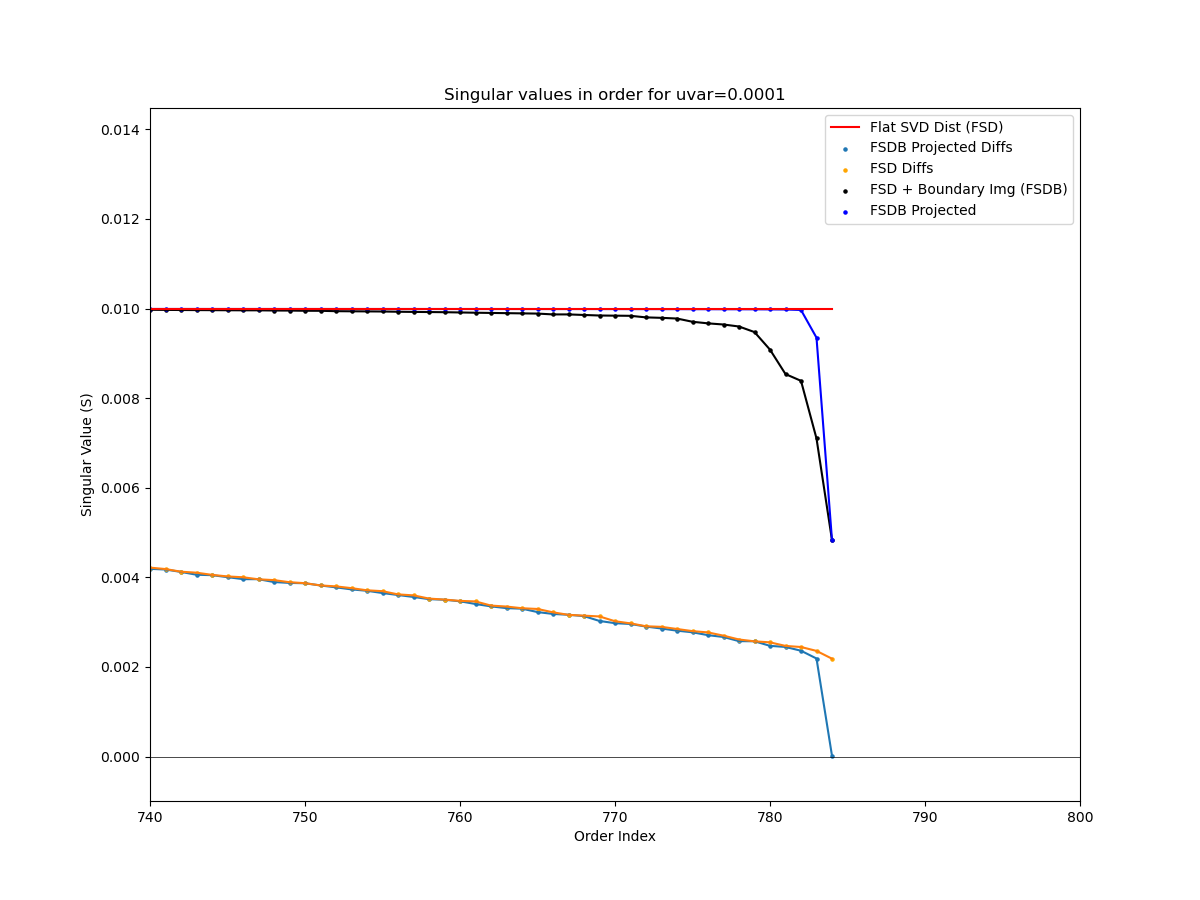
\includegraphics[width=14cm]{c4_figures/e06-SVD-uniform-rand_diff-decision_boundary_uvar-0.0001-index-0-image-999-cropped.png}

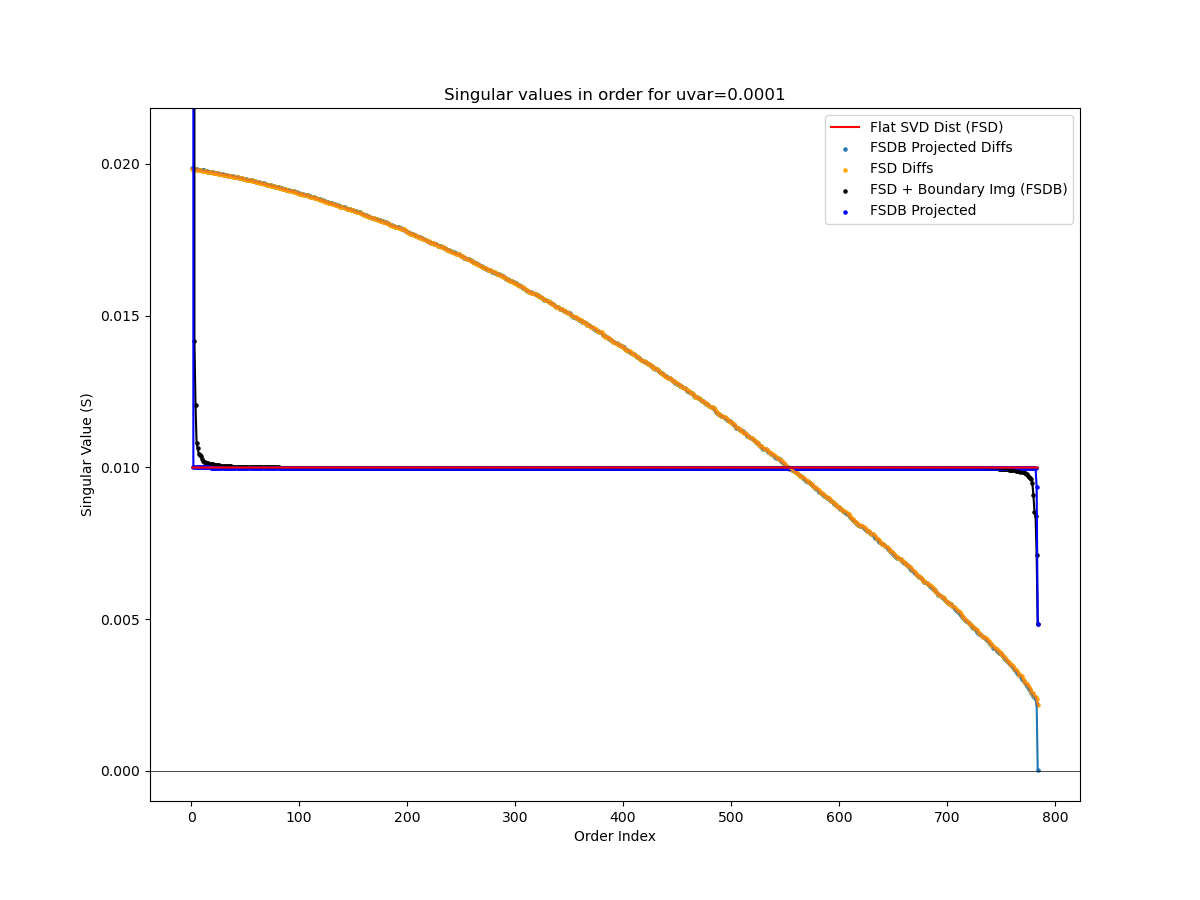
\includegraphics[width=14cm]{c4_figures/e06-SVD-uniform-rand_diff-decision_boundary_uvar-0.0001-index-0-image-999.png}

What these experiments tell us is that most of the time when we cross a decision oundary in the MNIST Dataset, we are crossing at a plane, however if we examine a slightly larger ball around a given point, it will intersect the decision boundary at many other places. 

\section{Re-Examining Persistence}

A movivating picture in this research is an image generated while interpolating persistence in the beginning of this research. 

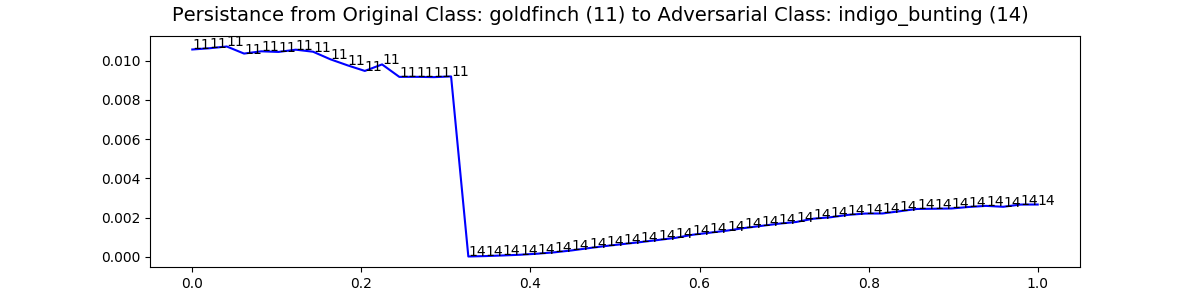
\includegraphics[width=15cm]{c4_figures/persistence_interpolation-IMNET-class-11-vgg16-BIM-48-attack_data-001 (2).png}

The next objective is to examine this particular case with our random walk and projection Tools. 

We also wish to augment these tools to include 

%%%%%%%%%%%%%%%%%

\subsection{in probability space}
\subsection{in image space}
\section{define orthants}
\section{skewness}

\section{sampling decision boundaries and analyzing dimensionality
with PCA}

\section{neural network attack gradients versus decision boundaries}

\section{skewed orthant recreates persistence picture (?). }
\section{measuring skewness of ANNs}
\section{Relate skewness with dimpled manifold and features not bugs papers}


turn observations into are they a definition, a theorem, or a discussion

decision\_boundary crossing

